Celem rozdziału jest przedstawienie środowiska programowania i bibliotek umożliwiających implementację kodu potrzebnych do stworzenia aplikacji internetowej z zastosowaniem urządzenia Raspberry Pi.

\section{Edytor kodu źródłowego}
W celu realizacji założeń projektowych, program został wykonany przy użyciu edytora kodu źródłowego Visual Studio Code. JavaScript jest językiem programowym, który znalazł uznanie wśród programistów. Udostępnia wiele gotowych bibliotek i frameworków, które można wykorzystać do tworzenia aplikacji. Visual Studio Code jest środowiskiem, które gwarantuje dobrą obsługę JavaScriptu i Node.js. Zapewnia narzędzia do podpowiadania składni i automatycznego uzupełniania kodu IntelliSense, a także narzędzia do debugowania i testowania aplikacji. Visual Studio Code również umożliwia korzystanie z niego na różnych systemach operacyjnych takich jak Linux czy Windows. Raspberry Pi ma wbudowany system operacyjny Linux dzięki czemu środowisko to idealnie się wkomponuje w tworzeniu aplikacji na tym urządzeniu. Aplikacja składa się z dwóch głównych elementów. Jest to serwer i klient. Część serwerowa to część aplikacji, która działa na serwerze i odpowiada za przetwarzanie i przechowywanie danych oraz obsługę żądań użytkowników. Została napisana w języku programowania JavaScript przy użyciu Node.js. Strona klienta to część aplikacji, która działa na urządzeniu użytkownika i odpowiada za wyświetlenie interfejsu użytkownika oraz komunikację z serwerem. Została ona napisana również w języku programowania JavaScript przy użyciu biblioteki React.js. Visual Studio Code pozwala na łatwą obsługę i zarządzanie strukturą plików co będzie pomocne przy tak dużych zasobach drzewa programu.

\section{Język JavaScript}
JavaScript jest językiem skryptowym. Jest on interpretowany przez środowisko uruchomienowe, którym może być przeglądarka lub Node.js. Umożliwia on tworzenie dynamicznych stron internetowych. Pozwala na projektowanie interfejsów użytkownika. JavaScript można używać w różnych aplikacjach gdzie wymagane jest sterowanie sprzętem czy serwerem. Z pomocą ogromnej społeczności wspierającej język, programiści mogą tworzyć aplikacje internetowe, czy przeznaczone na urządzenia przenośne. Pozwala tworzyć aplikacje i skrypty, które pozwolą na zarządzanie urządzenia Raspberry Pi. Istnieje wiele gotowych bibliotek, które umożliwiają połączenie i obsługę różnych elementów oraz urządzeń zewnętrznych podłączonych do mikrokontrolera. Sterowanie pinami GPIO przy użyciu języka programowania Javascript wymaga zaimportowania odpowiednich bibliotek. Język skryptowy jest zgodny z innymi systemami operacyjnymi w tym również z Linuxem, który jest domyślnym systemem operacyjnym dla Raspberry Pi.

\section{Node.js}
	Node.js jest środowiskiem uruchomieniowym opartym na języku JavaScript. Służy do budowy back-endu aplikacji oraz umożliwia uruchamianie kodu JavaScript poza przeglądarką internetową. Idealnie odnajduje swoje zastosowanie przy tworzeniu aplikacji sieciowych takich jak serwery internetowe. Node.js jest używany głównie do uzyskiwania dostępu do baz danych czy obsługi żądań. Środowisko Node.JS jest oparte o programowanie z wykorzystaniem zdarzeń. Dzięki temu, świetnie się sprawdza na urządzeniach o niewielkich zasobach, takich jak Raspberry Pi. Jest to spowodowane asynchroniczną naturą, która wymusza na programiście pisanie kodu nie blokującego główny wątek aplikacji. Jednocześnie, w przypadku zadań potrzebujących moc obliczeniową, może powodować to blokowanie obsługi innych zdarzeń. W ramach wykonywanej pracy, uznano że wykorzystanie zdarzeń oraz asynchronicznego oprogramowania będzie optymalnym doborem dla realizowanej aplikacji. Node.js został zaprojektowany do wykonania optymalizacji przepustowości i skalowalności w aplikacjach internetowych. Idealnie odnajduje swoje zastosowanie dla tworzenia aplikacji internetowych czasu rzeczywistego. Swoje działanie może zawdzięczać menadżerowi pakietów węzłów npm, który zapewnia dostęp do setek tysięcy pakietów i bibliotek. Express.js to biblioteka stworzona przy wykorzystaniu środowiska Node.JS, pozwalająca na obsługę żądań HTTP.  Jej głównym zadaniem jest udostępnianie szeregu narzędzi do obsługi protokołów sieciowych. Express.js stosuje się do tworzenia serwera sieciowego, który umożliwia komunikację między urządzeniami zewnętrznymi. Stworzona aplikacja internetowa jest pośrednikiem komunikacyjnym między maszyną, a użytkownikiem korzystającym z chatu. Celem zastosowania biblioteki Express.js jest możliwość udostępnienia wykonywania odpowiednich funkcji dostępnych na mikrokontrolerze Raspberry PI takich jak ustawienia stanu odpowiedniego pinu na płytce GPIO. Dzięki czemu, użytkownik może korzystać z modułów:
\begin{itemize}  
	\item \textbf{Moduł on-off}, umożliwia nam obsługę wejść/wyjść cyfrowych dla urządzeń zewnętrznych. Może być używany do sterowania diodami LED czy przełącznikami poprzez interfejsy takie jak GPIO, I2C lub SPI. Moduł on-off może być używany z systemem operacyjnym Windows czy Linux dzięki czemu idealnie odnajduje się przy programowaniu z użyciem Raspberry Pi. Zapewnia rejestrowanie zdarzeń zmiany stanu wejścia i wyjścia i pozwala reagować na nie. Dzięki temu modułowi jesteśmy w stanie integrować urządzenia zewnętrzne z aplikacjami Node.js, a także tworzyć projekty z wykorzystaniem Raspberry Pi i innych urządzeń z interfejsem GPIO.
	\\
	\item \textbf{Moduł pigpio}, biblioteka ta korzysta z frameworka Node.js. Moduł pigpio może być używany w celu kontrolowania i monitorowania sygnałów z wejść/wyjść cyfrowych. Umożliwia modulację szerokości impulsów na Raspberry Pi. Dzięki tej bibliotece jesteśmy w stanie tworzyć projekty z użyciem urządzeń elektronicznych takie jak diody LED czy serwomechanizmy, które są podłączone do określonych portów GPIO mikrokontrolera. Moduł ten znalazłaszerokie zastosowanie w aplikacjach gdzie wymagane jest sterowanie urządzeniami elektrycznymi lub elektronicznymi.
	\\
\end{itemize}

\section{React.js}
React.js to biblioteka Javascript, która swoje główne zastosowanie ma przy tworzeniu interfejsów użytkownika po stronie front-endu. Pozwala tworzyć dynamiczne aplikacje, w których interfejs użytkownika reaguje na zmiany wprowadzone w aplikacji. Swoje szerokie zastosowanie znajduje tam gdzie aplikacje opierają swoje funkcjonowanie na interakcjach użytkownika z elementami interfejsu użytkownika. React.js może idealnie współpracować z urządzeniem Raspberry Pi poprzez kontrolowanie urządzeń zewnętrznych podłączonych do tego urządzenia lub wyświetlania danych za pomocą stworzonego interfejsu. Umożliwia tworzenie interfejsu użytkownika za pomocą komponentów, które mogą być stosowane wielokrotnie przy projektowaniu różnych elementów. Główną zaletą stosowania React.js przy programowaniu z użyciem urządzenia Raspberry Pi jest tworzenie aplikacji, które muszą reagować na zmiany danych w czasie rzeczywistym.  
\newpage
\section{Wdrożenie aplikacji}
Relacja klient-serwer jest podstawowym modelem architektury systemów komputerowych, w którym oba te podmioty są różnymi urządzeniami bądź programami. Współpracują one ze sobą w celu umożliwienia użytkownikowi wymiany danych bądź korzystania z określonych usług. Aplikacje czasu rzeczywistego mają to do siebie, że serwer zazwyczaj odpowiada za przetwarzanie i przechowywanie danych oraz udostępnianie ich klientom. Klienci są odpowiedzialni za wyświetlenie tych danych i wykorzystanie ich według własnych założeń. Strona klienta i serwera komunikują się przy użyciu protokołów sieciowych takich jak WebSockets, aby umożliwić przepływ danych pomiędzy nimi. Aplikacje czasu rzeczywistego są często wykorzystywane w komunikacji tekstowej, aby pozwolić użytkownikom na szybką i efektywną wymianę informacji. Klienci mogą szybko uzyskać oczekiwaną odpowiedź z strony serwera po przesłaniu danego żądania, nie tracąc czasu na opóźnienia w przesyłaniu informacji. Takie aplikacje często znajdują swoje zastosowanie w sytuacjach, w których szybka i dokładna wymiana danych jest istotna. W stworzonej aplikacji, kluczowym elementem przesyłania żądania do mikrokontrolera jest uzyskanie jak najszybszej odpowiedzi urządzenia poprzez działanie elementów zainstalowanych po stronie mikrokomputera. Komunikacja przy pomocy relacji klient-serwer idealnie odnajduje swoje zastosowanie.

\newpage
\section{Model drzewa programu}
\begin{figure}[htbp]
	\centering
	\includegraphics[width=0.5\linewidth]{"obrazy/model"}
	\caption{Struktura programu}
	\label{fig:6}
\end{figure}
Struktura programu składa się z dwóch katalogów: 

\begin{itemize}  
	\item \textbf{ Klient}, odpowiedzialny za nawiązanie połączenia z serwerem oraz odbieranie i wysyłanie danych za pomocą Socket.IO. Po stronie klienta zaimplementowane są interfejsy użytkownika umożliwiające komunikacje z urządzeniem.
	\\
	\item \textbf{ Serwer}, odpowiedzialny za utrzymanie połączenia sieciowego z klientem i przesyłanie oraz odbieranie danych za pomocą Socket.IO. Serwer umożliwia odpowiadanie na żądania i przetwarzanie danych na odpowiednie czynności. Po stronie serwera zaimplementowany jest cały mechanizm umożliwiający komunikację tekstową. 
	\\
\end{itemize}
\section{Implementacja strony klienta}
Strona klienta została zaimplementowana przy użyciu biblioteki React.js, która służy przede wszystkim do tworzenia interfejsu użytkownika dla aplikacji internetowej. Główną zaletą korzystania z tego modułu jest możliwość tworzenia komponentów. Odpowiadają one za wyrenderowanie i zarządzanie fragmentem stworzonego widoku. Komponenty pozwalają na przedstawienie sposobu działania i wyglądu aplikacji. Są one w pełni niezależne od siebie co umożliwia ich wielokrotne użytkowanie w różnych miejscach aplikacji. Dzięki temu kod staje się bardziej modularny i łatwiejszy do zarządzania. Komponenty są tworzone za pomocą składni JSX, która umożliwia zapisanie kodu HTML w plikach JavaScript. W celu łatwiejszej implementacji interfejsów użytkownika zostało stworzone 6 komponentów:
\begin{itemize}  
	\item \textbf{ Logowanie}, komponent ten zwraca widok dołączenia użytkownika do komunikatora tekstowego. Jest on pierwszym interfejsem użytkownika podczas włączenia aplikacji.
	\\
	\item \textbf{ Czat}, komponent ten zwraca widok komunikatora tekstowego. Odpowiada za wysyłanie żądań do urządzenia.W jego skład wchodzą elementy nawigacji, zbioru wiadomości i komunikacji, które tworzą widok interfejsu użytkownika. 
	\\
\item \textbf{ Nawigacja}, komponent ten zwraca widok zawierający informacje o aktualnie wybranym pokoju przez użytkownika.
	\\
\item \textbf{ Komunikacja}, komponent ten zwraca widok zawierający pole tekstowe oraz przycisk wysyłania wiadomości w aplikacji.
	\\
\item \textbf{ Zbiór wiadomości}, komponent zwraca widok wyrenderowanej listy wiadomości
	\\
\item \textbf{ Wiadomość}, komponent ten zwraca widok wyrenderowania pojedynczej wiadomości
	\\
\end{itemize}
\newpage
\subsection{Komponent logowania}
\begin{figure}[htbp]
	\centering
	\includegraphics[width=0.5\linewidth]{"obrazy/logowanie"}
	\caption{Interfejs logowania}
	\label{fig:7}
\end{figure}

Komponent Logowania wyświetla formularz, w którym użytkownik może wprowadzić swoją nazwę i nazwę pokoju do którego chce dołączyć. Za pomocą przycisku „Sign In” może on przejść do komunikatora tekstowego. Nazwa użytkownika jest dowolna. Klient może dołączyć do pokoju, z którego korzystają już inni użytkownicy, a także może stworzyć swój własny oddzielny pokój. 


W komponencie logowania zaimplementowano funkcję zwracającą widok interfejsu użytkownika umożliwiającego dołączenie do czatu oraz dwie metody, które przechowują stany parametrów. Zmienne te pełnią ważną rolę podczas logowania użytkownika do aplikacji czatu. W nich przechowywana jest obecna wartość parametru nazwy pokoju i klienta. Umożliwiają one również rejestrowanie zmian tych dwóch stanów i dokonanie aktualizacji obecnej wartości parametru. W przypadku ustalenia nazwy użytkownika, metoda ta przechowuje obecną wartość wpisaną w polu tekstowym odpowiedzialnym za przechowywanie nazwy klienta korzystającego z aplikacji. Logując się ponownie do aplikacji jesteśmy w stanie zmieniać wartość tego pola i wpisywać nową nazwę użytkownika. Adekwatna sytuacja występuje również w przypadku metody służącej do przypisania nazwy pokoju. Komponent ten zwraca funkcję, która renderuje formularz. Zawiera on dwa pola tekstowe umożliwiającymi wprowadzenie nazwy użytkownika i pokoju komunikatora, a także przycisk logowania. Kiedy użytkownik wprowadzi swoją nazwę to obecny stan wartości zmiennej jest aktualizowany. Adekwatna sytuacja występuje przy wprowadzeniu nazwy pokoju. W komponencie zaimplementowano również mechanizm, który umożliwia przekierowanie użytkownika do strony komunikatora poprzez kliknięcie przycisku. Do spełnienia tej czynności, wymagane jest wypełnienie pola tekstowego z nazwą użytkownika i pokoju. Jeżeli jedno z tych sekcji jest niewypełnione, niemożliwe będzie przejście do komunikatora. Wymagane jest wpisanie obu danych w celu uzyskania dostępu do zalogowania.
\newpage
\begin{lstlisting}[caption=Implementacja komponentu logowania]
export default function SignIn() {
    const [name, setName] = useState('')
    const [room, setRoom] = useState('')

    return (
        <div className="joinOuterContainer">
            <div className="joinInnerContainer">
                <h1 className="heading">Chat</h1>
                <div>
                    <input
                        placeholder="Name"
                        className="joinInput"
                        type="text"
                        onChange={(event) =>
			 setName(event.target.value)}
                    />
                </div>
                <div>
                    <input
                        placeholder="Room"
                        className="joinInput mt-20"
                        type="text"
                        onChange={(event) =>
			 setRoom(event.target.value)}
                    />
                </div>
                {!name || !room ? null : (
                    <Link
                        onClick={(e) =>
                            !name || !room ?
			 e.preventDefault() : null
                        }
                        to={`/chat?name=${name}&room=${room}`}
                    >
                        <button className={'button mt-20'}
			 type="submit">
                            Sign In
                        </button>
                    </Link>
                )}
            </div>
        </div>
    )}
\end{lstlisting}
\newpage
\subsection{Komponent komunikatora}
\begin{figure}[htbp]
	\centering
	\includegraphics[width=0.7\linewidth]{"obrazy/komunikator"}
	\caption{Widok komponentu komunikatora}
	\label{fig:9}
\end{figure} 

Komponent czatu wyświetla komunikator tekstowy, w którym użytkownik może wprowadzać swoje żądania i komunikować się z maszyną. W jego skład wchodzą takie komponenty jak: 
\begin{itemize}  
\item \textbf{ Nawigacja}
	\\
\item \textbf{ Komunikacja}
	\\
\item \textbf{ Zbiór wiadomości}
	\\
\item \textbf{ Wiadomość}
\end{itemize}
Każdy z tych fragmentów interfejsu spełnia swoje założenia co pozwala na stworzenie widoku komunikatora. Komponent Nawigacji renderuje widok paska zawierającego nazwę pokoju oraz ikony z aktywnością pokoju i zamknięcia. Pierwsza z tych ikon wyświetlana jest zawsze i oznacza status dostępny w postaci zielonego koła. Po kliknięciu ikony zamknięcia zostaniemy ponownie przekierowany do komponentu logowania.
\begin{lstlisting}[caption=Implementacja komponentu nawigacji ]
const InfoBar = ({ room }) => (
  <div className="infoBar">
    <div className="leftInnerContainer">
      <img className="onlineIcon" src={onlineIcon} 
	alt="online icon" />
      <h3>{room}</h3>
    </div>
    <div className="rightInnerContainer">
      <a href="/"><img src={closeIcon} alt="close icon" /></a>
    </div>
  </div>);
\end{lstlisting}
Komponent Komunikacji służy do wysyłania wiadomości w aplikacji czatu. Element ten składa się z formularza zawierającego przycisk do wysyłania wiadomości i jedno pole tekstowe umożliwiające wpisanie wiadomości. Do komponentu przekazywane są 3 parametry odpowiedzialne za zarządzanie operacjami wysyłania wiadomości. Pozwalają one na aktualizację stanu tekstu wiadomości i przechowywanie aktualnej wartości wpisanej komendy. Podczas kliknięcia przycisku wywoływana jest funkcja odpowiedzialna za wysłanie wiadomości wpisanej w polu tekstowym.
\begin{lstlisting}[caption=Implementacja komponentu komunikacji ]
const Input = ({message,setMessage, sendMessage }) => (
        <form className='form'>
            <input 
                className='input'
                type="text"
                placeholder='Type a message...'
                value={message}
                onChange={(event) => 
		setMessage(event.target.value)}
                onKeyPress={(event) => event.key === 'Enter' ?
	 	sendMessage(event) : null }/>
            <button className='sendButton' 
		onClick={(e) => sendMessage(e)}><BiSend className='send' />
	</button>
        </form>
)
\end{lstlisting}
\newpage
Komponent o nazwie zbiór wiadomości renderuje nam widok wyświetlający listę wysłanych poleceń w aplikacji. Do elementu przekazywane są 2 parametry, które pozwalają na przekazywanie informacji o użytkowniku, który wysłał wiadomość. W komponencie zaimplementowany został element ScrollToBottom, który automatycznie przewija stronę do dołu, gdy dodawane są nowe wiadomości. Jest to wbudowana funkcja, udostępniana przez bibliotekę React.js. Za pomocą funkcji mapowania tworzone są  komponenty pojedynczej wiadomości dla każdego nowego wysłanego polecenia. Do wyrenderowanych elementów przekazywane są dwa parametry z komponentu zbioru wiadomości. Przypisywanie unikalnego klucza identyfikacji dla elementu pomaga systemowi w efektywnym zarządzaniu stanem aplikacji i wykrywaniu ewentualnych zmian w komponencie. 
\begin{lstlisting}[caption=Implementacja komponentu zbior wiadomosci ]
import ScrollToBottom from 'react-scroll-to-bottom';
const Messages = ({ messages, name }) => (
  
  <ScrollToBottom className="messages">
    {messages.map((message, i) => <div key={i}><Message
	 message={message} name={name}/></div>)}
  </ScrollToBottom>
);
\end{lstlisting}

Komponent Wiadomość wyświetla pojedyncze polecenie wysłane w aplikacji. Do elementu przekazywane są dwa parametry. Pozwalają one na zidentyfikowanie osoby, która przesyła komendy w komunikatorze. Również zaimplementowano mechanizm, który umożliwia zdefiniować czas i datę wysłania wiadomości przez użytkownika.
\newpage
\begin{lstlisting}[caption=Implementacja komponentu z pojedyncza wiadomoscia ]
const Message = ({ message: { text, user }, name }) => {
const [currentDate, setCurrentDate] = useState('')
    useEffect(() => {
        var date = new Date().getDate() 
        const monthNames = [
            'January',
            'February',
            'March',
            'April',
            'May',
            'June',
            'July',
            'August',
            'September',
            'October',
            'November',
            'December']
        let monthIndex = new Date().getMonth()
        let monthName = monthNames[monthIndex]
        var year = new Date().getFullYear() 
        var hours = new Date().getHours() 
        var min = new Date().getMinutes() 
        setCurrentDate(
            date+ ' '+ monthName+' '+year+', '+ hours+':'+min )
    }, [currentDate])
    let isSentByCurrentUser = false
    const trimmedName = name.trim().toLowerCase()
    if (user === trimmedName) {
        isSentByCurrentUser = true }
    return isSentByCurrentUser ? (
        <div className="messageContainer justifyEnd">
            <p className="sentText pr-10">{trimmedName}</p>
            <div className="messageBox backgroundBlue">
                <p className="messageText colorWhite">{text}</p>
                <p className="currentDate">{currentDate}</p>
            </div>
        </div>
    ) : (
        <div className="messageContainer justifyStart">
            <div className="messageBox backgroundLight">
                <p className="messageText colorDark">{text}</p>
                <p className="currentDate enemy">{currentDate}</p>
            </div>
            <p className="sentText pl-10 ">{user}</p>
        </div>)}
\end{lstlisting}
\newpage
\begin{figure}[htbp]
	\centering
	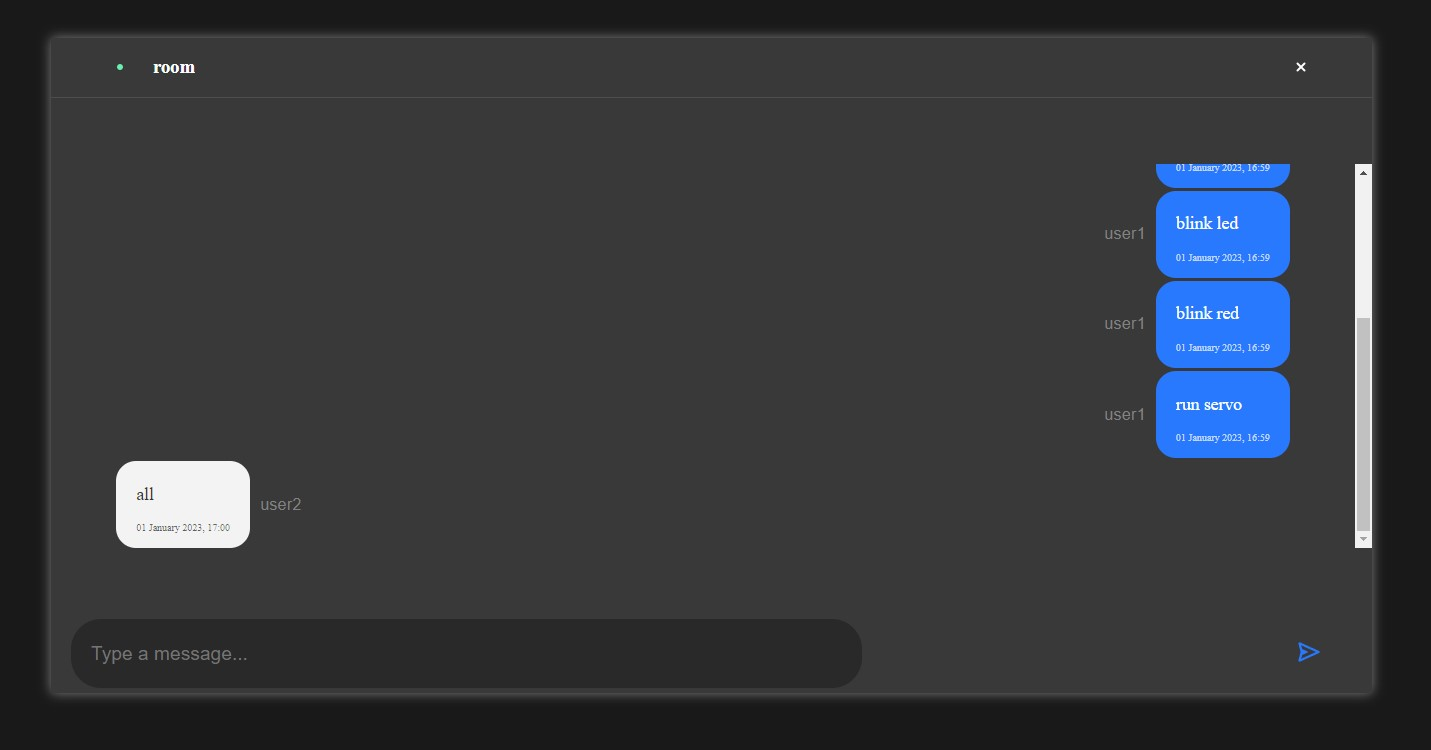
\includegraphics[width=0.5\linewidth]{"obrazy/interface2.jpg"}
	\caption{Widok komunikatora po wpisaniu wiadomości przez dwóch użytkowników}
	\label{fig:13}
\end{figure}
Do interfejsu komunikatora może dołączyć wiele osób. Mogą one wysyłać różne komendy. Pojawienie się wiadomości w komunikatorze podporządzkowane jest od tego czy została ona wysłana przez bieżącego użytkownika. W zależności od tego wyświetla ją w odpowiednim miejscu na ekranie - po lewej lub po prawej stronie. Wiadomość wysłana przez bieżącego użytkownika wyróżniona jest kolorem niebieskim. Komendy otrzymane od pozostałych klientów wyróżnione są kolorem szarym. Przy wpisanym poleceniu widać nazwę użytkownika, która tą wiadomość wysłała.

Komponent czat z użyciem Socket.IO umożliwia komunikację z mikrokontrolerem. W komponencie zadeklarowano parametry, które zarządzane są przez funkcje useState. Pozwalają one na zidentyfikowanie osoby, która bierze udział w komunikacji, a także określa wszystkie operacje, które wykonała. Za pomocą funkcji useEffect parsowane jest zapytanie z adresem URL. Następnie zapytanie te jest przekazywane do komponentu czatu poprzez parametr `location`. Po parsowaniu zapytania, wartości parametrów z nazwą użytkownika i pokoju używane są do przekierowania użytkownika na poprawny adres URL. Umożliwia to nawiązanie połączenia z serwerem. Przy zastosowaniu zdarzenia dołączenia, użytkownik zostaje przekierowany do komunikatora. Tam może nawiązywać komunikację tekstową z urządzeniem.

\begin{lstlisting}[caption=Implementacja funkcji dolaczenia do komunikatora po stronie klienta]
useEffect(() => {
        const { name, room } = queryString.parse(location.search)
        socket = io(ENDPOINT)
        setRoom(room)
        setName(name)
        socket.emit('join', { name, room }, (error) => {
            if (error) {
                alert(error)
            }})}, [ENDPOINT, location.search])
\end{lstlisting}

Aby użytkownik miał możliwość przesyłania komend do urządzenia potrzebne jest zaimplementowanie zdarzenia, które pozwoli na wysyłanie wiadomości. Konieczne jest, aby strona klienta mogła nasłuchiwać dane przychodzące z strony serwera. Przy wprowadzeniu nowej wiadomości przez użytkownika aktualizowany jest parametr odpowiadający za przechowywanie listy wysłanych poleceń. Powoduje to uaktualnienie danych klienta, który wysłał komendę w komunikatorze.
\begin{lstlisting}[caption=Implementacja funkcji nasluchiwania wiadomosci i danych przychodzacych od serwera]
useEffect(() => {
        socket.on('message', (message) => {
            setMessages((messages) => [...messages, message])
        })
        socket.on('roomData', ({ users }) => {
            setUsers(users)
        })
    }, [])
\end{lstlisting}

Aby użytkownik mógł przesłać polecenie, które pojawi się w interfejsie komunikatora, zaimplementowano funkcję odpowiadającą za wysyłanie wiadomości. Po wypełnieniu pola tekstowego i kliknięciu przycisku z symbolem wysłania następuje jej wywołanie. Zastosowano również mechanizm, który zapobiega automatycznemu renderowaniu się strony po przesłanym poleceniu w aplikacji. Serwer nasłuchuje zdarzenia wysłania wiadomości przychodzące z strony klienta i umożliwia wykonanie tej czynności. Kiedy użytkownik prześle komendę w aplikacji, zawartość tekstu jest usuwana umożliwiając ponowne wykonanie tej operacji
\begin{lstlisting}[caption=Implementacja funkcji do wysylania wiadomosci]
const sendMessage = (event) => {
        event.preventDefault()
        if (message) {
          socket.emit('sendMessage',message,()=>setMessage(''))
       	}}
\end{lstlisting}

Wszystkie te komponenty wchodzą w skład tworzenia interfejsu użytkownika. Widok ten pełni funkcję komunikatora z mikrokontrolerem. Użytkownik może wysyłać wiadomości napisane w języku naturalnym do urządzeń za pomocą interfejsu komunikatora. Poprzez zdalne skonfigurowanie Raspberry Pi, mikrokontroler będzie odbierał polecenia z aplikacji czatu i wykonywał będzie operacje odpowiadające między innymi za włączenie lub wyłączenie elementów wykonawczych podłączonych do określonych portów GPIO.
\newpage
\begin{lstlisting}[caption=Implementacja komponentu czatu]
const Chat = ({ location }) => {
    const [name, setName] = useState('')
    const [room, setRoom] = useState('')
    const [users, setUsers] = useState('')
    const [message, setMessage] = useState('')
    const [messages, setMessages] = useState([])

	....	

    return (
        <div className="outerContainer">
            <div className="container">
                <InfoBar room={room} />
                <Messages messages={messages} name={name} />
                <Input
                    message={message}
                    setMessage={setMessage}
                    sendMessage={sendMessage}
                />
            </div>
        </div>
    )
}
\end{lstlisting}
\section{Zarządzanie ścieżką nawigacji}
Ważnym aspektem w aplikacji jest również możliwość tworzenia trasy między komponentami i wędrowanie pomiędzy nimi. Każdy komponent zawiera adres URL, który odpowiada określonemu widokowi w aplikacji. Za pomocą biblioteki ‘react-router-dom’ możemy tworzyć ścieżkę nawigacji wskazująca, który interfejs ma zostać wyświetlony na stronie w odpowiedzi na zmianę adresu URL bez konieczności przeładowywania całej strony.
\begin{lstlisting}[caption=Implementacja sciezki nawigacji pomiedzy interfejsami]
const App = () => {
  return (
    <Router>
      <Route path="/" exact component={Join} />
      <Route path="/chat" component={Chat} />
    </Router>
  );
}
\end{lstlisting}
Aby móc wędrować pomiędzy komponentami logowania i czatu konieczne było stworzenie trasy z wyznaczoną ścieżką docelową. Komponent nawigacji umożliwia aplikacji reagowanie na zmianę adresu URL w przeglądarce internetowej. Każdy z tych interfejsów zawiera swoją wyznaczoną ścieżkę, która jest potrzebna przy zmianie widoku aplikacji przez użytkownika. Zaimplementowana nawigacja przekierowuje nas do interfejsu komunikatora po wprowadzeniu nazwy użytkownika i nazwy pokoju w komponencie logowania. Znajdując się w interfejsie komunikatora, również możemy wrócić z powrotem do komponentu logowania poprzez kliknięcie przycisku zamknięcia. Znajduje się on w prawym górnym rogu okienku czatu.
\section{Implementacja strony serwera}
Strona serwera została zaimplementowana przy użyciu środowiska uruchomieniowego Node.js. Umożliwia ono tworzenie szybkich i skalowalnych aplikacji sieciowych za pomocą języka JavaScript. Node.js używa modelu jednowątkowego do obsługi wielu żądań jednocześnie co oznacza, że jest on idealny do tworzenia aplikacji sieciowych takich jak serwery czy komunikatory tekstowe. Ważnym aspektem przy korzystaniu z środowiska uruchomieniowego Node.js jest możliwość tworzenia aplikacji w czasie rzeczywistym. Po stronie serwera zaimplementowany został cały mechanizm komunikacji z naszą maszyną, która umożliwia przede wszystkim przesyłanie oraz odbieranie danych.
Biblioteka Express.js  jest narzędziem sieciowym dla Node.js, która umożliwia tworzenie aplikacji opartych na serwerze. Express.js umożliwia obsługę żądań oraz mapowanie adresów URL na odpowiednie funkcje obsługujące te żądania. Głównym zastosowaniem biblioteki express.js jest możliwość tworzenia serwera HTTP, który będzie odpowiadał na żądania aplikacji klienckich. Biblioteka express.js znajduje swoje szerokie zastosowanie przy tworzeniu aplikacji serwerowych. Poza możliwością tworzenia serwera http, express.js umożliwia również obsługę różnych żądań czy parsowanie przesyłanych żądań. Możliwa jest również obsługa sesji użytkowników, autoryzację, a także przechowywanie i udostępnianie danych.
Node.js oferuje nam biblioteki http i express, które umożliwiają stworzenie serwera. Przy użyciu protokołu sieciowego tworzona jest jego instancja. Strona serwera nasłuchuje zdarzenia na wybranym porcie i loguje informację o uruchomieniu. Port to numer identyfikujący aplikację. Przy tworzeniu serwera konieczne jest ustalenie numeru portu, na którym możliwe będzie nasłuchiwanie i odbieranie połączeń od klientów. Użytkownicy mogą wysyłać zapytania do serwera poprzez podanie adresu IP serwera i numeru portu. Serwer odpowiada na żądania klientów poprzez wysłanie danych z powrotem do użytkownika poprzez ten sam port. Przy pomocy biblioteki express, serwer będzie nasłuchiwał żądań i odpowiadać na nie. 
\newpage
\begin{lstlisting}[caption=Implementacja serwera]
const http = require('http')
const express = require('express')
const socketio = require('socket.io')
const cors = require('cors')
const PORT = process.env.PORT || 5000
const app = express()
const server = http.createServer(app)
const io = socketio(server)
....
server.listen(PORT, () => console.log(`Server has started on port 
${PORT}`))
\end{lstlisting}
Poprzez zastosowanie biblioteki express.js możliwe jest utworzenie modułu ścieżki nawigacji przy wysyłaniu żądań. Obiekt ten służy do mapowania adresów URL z odpowiednimi funkcjami obsługi żądań. Moduł ten zawiera definicję trasy, która odpowiada żądaniom typu GET. Metoda ta stosowana jest w celu pobierania danych z serwera kiedy z nim się połączymy.
\begin{lstlisting}[caption=Implementacja sciezki serwera]
const express = require("express");
const router = express.Router();
router.get("/", (req, res) => {
  res.send("Server is up and running");
});
module.exports = router;
\end{lstlisting}
\section{Obsługa zdarzeń}
Obsługa zdarzeń po stronie serwera to proces reagowania na zdarzenia, które występują w aplikacji. Przykłady takich zdarzeń obejmują żądania HTTP od użytkowników czy otrzymanie danych za pośrednictwem protokołu sieciowego. Aby obsłużyć zdarzenie po stronie serwera należy utworzyć zdarzenia nasłuchiwania, które w odpowiedzi wykonują określone zadania.
\subsection{Zdarzenia nasłuchiwania}
W celu odbierania zapytań od klientów i wysyłania odpowiedzi zwrotnych implementuje się zdarzenie nasłuchiwania po stronie serwera. Gdy serwer jest uruchomiony i nasłuchuje na określonym porcie, może otrzymywać zapytania od klientów poprzez wysyłanie danych na ten port. Serwer może obsługiwać wiele różnych żądań od klientów jednocześnie, dlatego implementuje się zdarzenie nasłuchiwania, które jest wywoływane za każdym razem gdy serwer otrzyma nowe żądanie od klienta. Zdarzenie to umożliwia serwerowi reagowanie na żądania klienta poprzez wysyłanie odpowiedzi zwrotnej. 
Przy pomocy biblioteki Socket.IO rejestrowane jest zdarzenie dołączenia do komunikatora. Funkcja ta wywoływana jest za każdym razem kiedy użytkownik wyśle żądanie do serwera z możliwością dołączenia do pokoju czatu. Następnie emitowane jest zdarzenie zawierające obiekt z danymi o pokoju i zalogowanych użytkownikach.
\begin{lstlisting}[caption=Implementacja zdarzenia dolaczenia i pobierania danych]
io.on('connection', (socket) => {
  socket.on('join', ({ name, room }, callback) => {
    const { error, user } = addUser({ id: socket.id, name, room})
    if (error) return callback(error)
    socket.join(user.room)
    io.to(user.room).emit('roomData', {
    room: user.room,
    users: getUsersInRoom(user.room),
      })
         ....		
        callback()
    })
	....
})
\end{lstlisting}

Żeby zdarzenie dołączenia mogło być realizowane potrzebne jest zaimplementowanie operacji dodawania nowego klienta. Jest to potrzebne, żeby serwer mógł aktualizować listę użytkowników zarejestrowanych w aplikacji oraz nasłuchiwać wysyłane żądania. Przy pomocy funkcji dodawany jest nowy klient do listy użytkowników. W tym celu pobierana jest jego nazwa, nazwa pokoju, w którym się znajduje, a także unikalny klucz identyfikatora.
\begin{lstlisting}[caption=Implementacja funkcji dodawania uzytkownika]
const addUser = ({ id, name, room }) => {
    name = name.trim().toLowerCase()
    room = room.trim().toLowerCase()
    const existingUser = users.find(
        (user) => user.room === room && user.name === name
    )
    const user = { id, name, room }
    users.push(user)
    return { user }
}
\end{lstlisting}
W celu umożliwienia wysyłania wiadomości przez użytkowników, implementuje się po stronie serwera zdarzenie wysyłania wiadomości. Funkcja ta jest wywoływana, gdy żądanie zostanie wyrejestrowane. Kiedy klient wysyła wiadomość do serwera, ten odbiera to zdarzenie i uruchamiana jest funkcja. Następnie serwer pobiera informacje o użytkowniku, który przesłał polecenie i emituje zdarzenie wiadomości do wszystkich użytkowników znajdujących się w tym samym pokoju. Funkcja ta działa jako most między klientem, a serwerem, umożliwiając im wymianę danych.
\begin{lstlisting}[caption=Implementacja zdarzenia wysylania wiadomosci]
socket.on('sendMessage', async (message, callback) => {
        const user = getUser(socket.id)
        	....
        io.to(user.room).emit('message', {
            user: user.name,
            text: message,
            createdTime,
        })

        callback()
    })
}
\end{lstlisting}
Do realizacji zdarzenia wysłania wiadomości, konieczne jest zidentyfikowanie, który użytkownik wykonał tą operacje. W tym celu pobierane są dane użytkownika po przypisanym unikalnym kluczu identyfikatora. Sprawdzane jest czy identyfikator użytkownika z tablicy jest równy identyfikatorowi przekazanemu jako argument użytkownika. Jeżeli warunek zostanie spełniony to następuje zwrócenie obiektu użytkownika, który wysłał wiadomość.
\begin{lstlisting}[caption=Implementacja funkcji pobierania informacji o uzytkowniku]
const getUser = (id) => users.find((user) => user.id === id)
\end{lstlisting}

Również zaimplementowano zdarzenie rozłączania, które jest potrzebne do aktualizowania liczby uczestników korzystających z aplikacji. Funkcja ta jest wywoływana kiedy użytkownik rozłączy się z serwerem. Usuwane są informacje o użytkowniku z listy użytkowników i następnie wysyłany jest komunikat do pozostałych uczestników, informujący o jego opuszczeniu. Po rozłączeniu się klienta, aktualizowana jest lista użytkowników w pokoju.
\newpage
\begin{lstlisting}[caption=Implementacja zdarzenia rozlaczania]
socket.on('disconnect', () => {
        const user = removeUser(socket.id)
        if (user) {
            io.to(user.room).emit('message', {
                user: 'Admin',
                text: `${user.name} has left.`,
            })
            io.to(user.room).emit('roomData', {
                room: user.room,
                users: getUsersInRoom(user.room),
            })
        }})
\end{lstlisting}

W celu aktualizacji listy użytkowników zaimplementowano metodę, która pozwoli na wykonanie tej operacji. Funkcja iteruje po tablicy obecnych użytkowników w pokoju, sprawdzając czy nazwa pokoju użytkownika jest zgodna z nazwą pokoju przekazanej do funkcji jako argument. Jeśli tak to użytkownik dodawany jest do nowej tablicy.
\begin{lstlisting}[caption=Implementacja funkcji aktualizujaca liste uzytkownikow]
const getUsersInRoom = (room) => users.filter((user) => 
user.room === room)
\end{lstlisting}

Żeby zdarzenie rozłączenia mogło być realizowane, potrzebne jest zaimplementowanie operacji usuwania użytkownika. Funkcja w celu sprawdzenia, który użytkownik opuścił czat, przyjmuje parametr identyfikatora. Przypisywany jest on każdemu użytkownikowi. Warunkiem jest sprawdzenie czy identyfikator przekazanego argumentu jako argument użytkownika jest zgodny z klientem znajudjącym się na liście.Jeśli tak, to zwracany jest indeks tego elementu co powoduje usunięcie użytkownika z listy. 
\begin{lstlisting}[caption=Implementacja funkcji usuwania uzytkownika]
const removeUser = (id) => {
    const index = users.findIndex((user) => user.id === id)
    if (index !== -1) return users.splice(index, 1)[0]
}
\end{lstlisting}
\newpage
\section{Translacja komend do komunikacji z mikrokontrolerem}
W celu umożliwienia komunikacji tekstowej z maszyną za pomocą aplikacji, potrzebne jest nasłuchiwanie zdarzeń wysyłania wiadomości przez serwer. Kiedy klient wysyła żądanie do serwera, ten pobiera informacje o wysłanej wiadomości. Następnie emituje ją w celu komunikacji z mikrokontrolerem.  Potrzebna jest lista komend napisanych w języku naturalnym, które będą odpowiadać wpisanym w aplikacji wiadomościom. Odpowiedzialne one będą za zadziałanie danego elementu wykonawczego podłączonego do mikrokontrolera.
\begin{lstlisting}[caption=Translacja komend na odpowiednie funkcje]
socket.on('sendMessage', async (message, callback) => {
        const user = getUser(socket.id)
        switch (message) {
            case 'blink red': {
                blinkRed()
                break
            }
            case 'turn on all': {
                turnOnAll()
                break
            }
            case 'turn off all': {
                turnOffAll()
                break
            }
            case 'sequential': {
                sequential()
                break
            }
            case 'sensor': {
                sensor()
                break
            }
            case 'run servo': {
                servo()
                break
            }
            case 'flowing leds': {
                flowingLeds()
                break
            }
            case 'stop yellow': {
                endBlinkYellow()
                break
            }
            case 'yellow on': {
                tryYellow()
                break
            }
            case 'blink yellow': {
                blinkYellow()
                break
            }
            case 'stop green': {
                endBlinkGreen()
                break
            }
            case 'green on': {
                tryGreen()
                break
            }
            case 'blink green': {
                blinkGreen()
                break
            }
            case 'red on': {
                tryRed()
                break
            }
            case 'stop red': {
                endBlinkRed()
                break
            }}
	...
        callback()
    })
\end{lstlisting}

Gdy serwer otrzyma polecenie od klienta, sprawdzi co ta wiadomość zawiera i wywoła odpowiednią funkcję. Do implementacji określonych akcji w zależności od wprowadzonego wyrażenia zastosowano instrukcję switch-case. Jest to konstrukcja decyzyjna, która umożliwia dokonanie wyboru spośród przypisanych opcji. Jeśli znaleziono pasującą wartość, kod zostanie wykonany dla tego przypadku. Instrukcja „switch” sprawdza przypisaną zmienną i porównuje ją z poszczególnymi przypadkami. Gdy zostanie odnaleziona pasująca opcja, realizowane będzie działanie dla tego przypadku. Instrukcja ta ma nieograniczony wybór opcji i zależna jest od projektanta. Dla parametru odpowiedzialnego za przechowywanie wartości wpisanej wiadomości, zostały przypisane komendy napisane w języku naturalnym. Przy pomocy zastosowanej instrukcji sprawdzana jest pasująca wiadomość, która odpowiedzialna jest za wywołanie danej funkcji. Następnie serwer nasłuchuje zdarzenie wysyłania wiadomości i przy komunikacji z urządzeniem Raspberry Pi, uruchamiany jest dany element elektroniczny. Jeżeli zostanie wpisana komenda, która nie znajduje się ujęta w instrukcji to zostanie zwrócona bez jakichkolwiek działań.

\subsection{Włączenie diody LED}
By umożliwić komunikację elementów elektronicznych z mikrokontrolerem należy je podłączyć do odpowiednich wyprowadzeń pinów GPIO. Poprzez zastosowanie biblioteki ‘onOff’ tworzony jest obiekt LED. Dioda o kolorze czerwonym została podłączona do pinu 4 jako wyjście. Sprawdzane jest kolejno czy stworzony obiekt ma wartość 0 co oznacza to, że element nie jest aktywny. Jeśli tak, to zmieniany jest stan na wyjściu na wartość równą 1 co powoduje zaświecenie diody LED. Identyczna funkcja zaimplementowana jest również dla dwóch pozostałych diod.
\begin{lstlisting}[caption=Implementacja funkcji wlaczajacej diode]
function tryRed() {
    var LED = new onOff.Gpio(4, 'out')
    return new Promise((resolve) => {
        setTimeout(() => {
            if (LED.readSync() === 0) {
                LED.writeSync(1)
            }}, 10)
        resolve()
    })}
\end{lstlisting}

\subsection{Wyłączenie diody LED}
W celu kontrolowania diody LED, zaimplementowano również funkcję, która pozwoli na jej wyłączenie. Jej sposób działania jest niemal identyczny co do włączenia elementu, tylko w przypadku wyłączenia, stan jest zmieniany z wartości 1 na 0. Element usuwany jest z listy eksportowanych pinów i po odłączeniu obiektu LED, zostaje on wyłączony.
\begin{lstlisting}[caption=Implementacja funkcji wylaczajacej diode]
function endBlinkRed() {
    var LED = new onOff.Gpio(4, 'out')
    return new Promise((resolve) => {
        setTimeout(() => {
            LED.writeSync(0)
            LED.unexport()
            resolve()
        }, 3000)
    })}
\end{lstlisting}
\newpage
\subsection{Włączenie wszystkich diod}
W celu umożliwienia włączenia trzech diod LED stworzono nowe obiekty odpowiadające elementom. Zostały one podłączone do określonych pinów GPIO na wyjście układu. Sprawdzane jest kolejno czy stworzone obiekty mają wartość 0. Oznacza to, że elementy są nieaktywne. Jeśli tak, to zmieniany jest stan na wyjściu na wartość równą 1. Powoduje to zaświecenie wszystkich trzech diod.
\begin{lstlisting}[caption=Implementacja funkcji włączająca wszystkie diody]
function turnOnAll() {
    var LED04 = new onOff.Gpio(4, 'out'),
        LED17 = new onOff.Gpio(17, 'out'),
        LED27 = new onOff.Gpio(27, 'out')
        return new Promise((resolve) => {
        setTimeout(() => {
            if (
                LED04.readSync() === 0 &&
                LED17.readSync() === 0 &&
                LED27.readSync() === 0
            ) {
                LED04.writeSync(1)
                LED17.writeSync(1)
                LED27.writeSync(1)
            }}, 1)
        resolve()
})}
\end{lstlisting}

\subsection{Wyłączenie wszystkich diod}
W celu umożliwienia wyłączenia wszystkich trzech diod LED, sprawdzane jest czy zaimplementowane obiekty mają wartość 1 na wyjściu. Oznacza to, że elementy są włączone i się świecą. Jeśli tak, to zmieniany jest stan na wyjściu na niski co powoduje wyłączenie wszystkich trzech diod. 
\newpage
\begin{lstlisting}[caption=Implementacja funkcji wyłączająca wszystkie diody]
function turnOffAll() {
    var LED04 = new onOff.Gpio(4, 'out'),
        LED17 = new onOff.Gpio(17, 'out'),
        LED27 = new onOff.Gpio(27, 'out')
        return new Promise((resolve) => {
        	setTimeout(() => {
	            LED04.writeSync(0)
	            LED17.writeSync(0)
	            LED27.writeSync(0)
	            LED04.unexport()
	            LED17.unexport()
	            LED27.unexport()
	            resolve()
        }, 3000)})}
\end{lstlisting}

\subsection{Naprzemienne włączanie diod}
Aby umożliwić obsługę 3 diod LED, należy je podłączyć do trzech osobnych pinów GPIO. Czynność ta będzie potrzebna do osiągnięcia efektu płynącej diody. Wykonanie tej operacji ma na celu stworzenie wizualnego efektu ruchu elementów. Możliwe jest to do osiągnięcia przy zastosowaniu szeregu diod LED, które są sekwencyjnie zapalane. W celu realizacji takiego efektu tworzone są trzy obiekty, które odpowiedzialne będą za zarządzanie pinami GPIO o numerach, 4,17 i 27. Następnie zapisywane są do tablicy i zerowany jest ich stan. W zależności od aktualnego indeksu utworzonej tablicy, zmieniana jest wartość stanu z 0 na 1 co powoduje włączenie diody. W momencie osiągnięcia pozycji ostatniego elementu tablicy, zmieniany jest kierunek włączania diod. Przy zastosowaniu funkcji interwałowej, możliwe jest powtarzanie się czynności włączania i wyłączania elementów o określony czas. Daje to efekt wizualnego ruchu diod. Po upływie 5 sekund, elementy usuwane są z listy eksportowanych pinów co powoduje odłączenie obiektu i zakończenie procesu.
\newpage
\begin{lstlisting}[caption=Implementacja funkcji tworzącej efekt płynącej diody]
function flowingLeds() {
    var LED04 = new onOff.Gpio(4, 'out'),
        LED17 = new onOff.Gpio(17, 'out'),
        LED27 = new onOff.Gpio(27, 'out')
    var leds = [LED04, LED17, LED27]
    var indexCount = 0
    dir = 'up'
    return new Promise((resolve) => {
        var flowInterval = setInterval(flowingLeds, 300)
        function flowingLeds() {
            leds.forEach(function (currentValue) {
                currentValue.writeSync(0)
            })
            if (indexCount == 0) dir = 'up'
            if (indexCount >= leds.length) dir = 'down'
            if (dir == 'down') indexCount--
            leds[indexCount].writeSync(1)
            if (dir == 'up') indexCount++
        }
        setTimeout(() => {
            clearInterval(flowInterval)
            leds.forEach(function (currentValue) {
                currentValue.writeSync(0)
                currentValue.unexport()
                resolve()
            })}, 5000)
    })}
\end{lstlisting}

\subsection{Miganie diodą LED}
Aby uzyskać efekt migającej diody LED zaimplementowano funkcję wykorzystująca interwał czasowy. W tym celu utworzono obiekt, który został podłączony do pinu GPIO o numerze 4. Identyczna sekwencja została wykonana dla dwóch kolejnych diod o kolorze zielonym i żółtym. Za pomocą utworzonej funkcji sprawdzany jest stan diody. Jeżeli dioda jest wyłączona to zmieniany jest stan na wartość 1 co powoduje włączenie się elementu. Poprzez zastosowanie interwału czasowego możliwe jest powtarzanie się czynności co 250 milisekund. Powoduje to utworzenie efektu migającej diody LED.
\newpage
\begin{lstlisting}[caption=Implementacja funkcji tworząca efekt migania pojedynczej diody LED]
function blinkRed() {
    const LED = new onOff.Gpio(4, 'out')
    return new Promise((resolve) => {
        const blinkInterval = setInterval(blinkLED, 250)
        function blinkLED() {
            if (LED.readSync() === 0) {
                LED.writeSync(1)
            } else {
                LED.writeSync(0)
            }}
        setTimeout(() => {
            clearInterval(blinkInterval)
            LED.writeSync(0)
            LED.unexport()
            resolve()
        }, 5000)
    })}
\end{lstlisting}
\subsection{Sterowanie serwomechanizmem}
Serwomechanizm to układ, który pozwala na precyzyjne pozycjonowanie elementu względem określonego punktu. Mechanizm ten składa się z silnika elektrycznego, przekładni i elementu ruchomego. W momencie gdy kontroler serwomechanizmu otrzymuje sygnał o zadanej pozycji, silnik obraca się w odpowiednim kierunku. W celu cyklicznego włączaniu i wyłączaniu sygnału elektrycznego można zastosować technikę modulacji szerokością impulsu. Sterowanie serwomechanizmem przy pomocy sygnałów PWM polega na cyklicznym podawaniu impulsu o zmiennej szerokości. Silnik serwomechanizmu jest wówczas włączany i wyłączany w odpowiednim momencie, co pozwala na uzyskanie pożądanego położenia elementu.
\newpage
\begin{lstlisting}[caption=Implementacja funkcji sterująca serwomechanizmem]
function servo() {
    return new Promise((resolve) => {
        let pulseWidth = 1000
        const threshold = 20
        let increment = threshold
        const servoInterval = setInterval(() => {
            motor.servoWrite(pulseWidth)
            pulseWidth += increment
            if (pulseWidth >= 2000) {
                increment = -1 * threshold
            } else if (pulseWidth <= 1000) {
                increment = threshold
            }
        }, threshold)
        setTimeout(() => {
            clearInterval(servoInterval)
            resolve()
        }, 20000)
    })}
\end{lstlisting}
W celu spełnienia założeń przy sterowaniu serwomechanizmem zaimplementowano funkcję. Wykorzystuje ona technikę sterowania sygnałami PWM. Przy zastosowaniu interwałów czasowych, szerokość impulsów zwiększa się co określoną jednostkę czasową. Jeżeli serwomechanizm osiągnie pozycję końcową następuje zmniejszanie się wartości szerokości impulsu przez co serwomechanizm zacznie się cofać do pozycji początkowej. Czynność ta jest powtarzana przez 20 sekund. Po tym czasie następuje wyczyszczenie interwału czasowego co zatrzymuje działanie serwomechanizmu.
\subsection{Sekwencyjne wykonywanie komend}
W celu implementacji sekwencyjnego uruchamiania elementów podłączonych do pinów GPIO mikrokontrolera zastosowano asynchroniczne funkcje. Sekwencyjne wywoływanie funkcji to sposób, który umożliwi wykonywanie zaimplementowanych metod po kolei. Kiedy jedna funkcja zostanie zakończona, następuje wywołanie kolejnej. Zastosowanie asynchronicznego mechanizmu pozwoli na zaimplementowanie funkcji, które będą się wykonywały jedna po drugiej. Kiedy pierwsza operacja zrealizuje swoją pracę, informacja o jej zakończeniu zostanie przekazana do kolejnej funkcji, która następnie wykona swoją pracę. Pozwoli to na osiągnięcie efektu sekwencyjnego wykonywania się poleceń. 
\newpage
\begin{lstlisting}[caption=Sekwencyjne uruchamianie się funkcji]
async function sequential() {
    await turnOnAll()
    await turnOffAll()
    await tryRed()
    await endBlinkRed()
    await tryGreen()
    await endBlinkGreen()
    await tryYellow()
    await endBlinkYellow()
    await flowingLeds()
    await blinkRed()
    await blinkGreen()
    await blinkYellow()
    await servo()
}
\end{lstlisting}
\newpage
\section{Projektowanie układu działania}
Płytka prototypowa umożliwia połączenie elementów elektronicznych do pinów GPIO mikrokontrolera. Poprzez wpisanie określonych komend w aplikacji, możliwe będzie wysyłanie poleceń do Raspberry Pi. Będą one odpowiedzialne za wykonywanie operacji na podłączonych urządzeniach wykonawczych. W celu sprawdzenia funkcjonalności komunikacji tekstowej zaprojektowano stanowisko układu, w którego skład wchodzą elementy takie jak: 
\begin{itemize}  
	\item \textbf{Dioda LED koloru czerwonego}, anoda tego elementu została podłączona do pinu GPIO 4, zaś katoda do pinu GND
	\\
\item \textbf{Dioda LED koloru zielonego}, anoda tego elementu została podłączona do pinu GPIO 17, zaś katoda do pinu GND
	\\
\item \textbf{Dioda LED koloru żółtego}, anoda tego elementu została podłączona do pinu GPIO 27, zaś katoda do pinu GND
	\\
	\item \textbf{Serwomechanizm}, zasilanie tego elementu zostało podłączone do pinów +5V i GND. Pin sygnałowy został podłączony do pinu MOSI
	\\
\end{itemize}
Wraz z diodą LED szerogowo podłączono rezystor. Służy on do ogarniczenia prądu płynącego przez obwód. Raspberry Pi jest przystosowane do pracy z niskim obciążeniem prądowym. W takim przypadku dioda będzie przepuszczać prąd tylko w jednym kierunku. Oznacza to, że jeżeli wartość prądu będzie zbyt wysoka to dioda się zablokuje i ograniczy jego przepływ. Uchroni pozostałe elementy obwodu przed uszkodzeniem. Ważne jest dobranie odpowiedniej wartości rezystora. Zależna jest od napięcia zasilania, napięcia przewodzenia i od prądu elementu. Podczas sterowania diodą LED, Raspberry Pi wysyła sygnał sterujący do pinu, który jest połączony z anodą elementu. Sygnał ten przechodzi przez rezystor ograniczający prąd. Następnie płynie przez obiekt powodując jego zaświecenie.

Serwomechanizm służy do precyzyjnego sterowania położeniem obrotowego elementu. Raspberry Pi wysyła sygnał sterujący do serwomechanizmu za pomocą odpowiedniego interfejsu takiego jak PWM. Pozwala on na regulację prędkości i położenia silnika. Wysyłany sygnał odpowiada za ruch elementu i generowany jest na podstawie informacji o pozycji zadanej. Mikrokontroler monitoruje położenie silnika i dostosowuje sygnał sterujący, aby zapewnić precyzyjne położenie elementu.



\newpage
\begin{figure}[h]
\begin{subfigure}{0.5\textwidth}
\includegraphics[width=0.9\linewidth, height=6cm]{"obrazy/ukladpolaczenia3"} 

\end{subfigure}
\begin{subfigure}{0.5\textwidth}
\includegraphics[width=0.9\linewidth, height=6cm]{"obrazy/ukladpolaczenia2"}

\end{subfigure}

\caption{Układ połączenia elementów wykonawczych}
\label{fig49}
\end{figure}

\section{Archiwizacja wpisanych poleceń}
Celem archiwizacji wiadomości jest możliwość przeglądania przez użytkownika historii komend wykonanych w aktualnej lub poprzedniej sesji. Z ich pomocą użytkownik wie, czy dana komenda została już wykonana, a jeżeli tak to kiedy oraz kto ja wykonał. Historia wiadomości może okazać się ważna w przypadku nieoczkiwanego przerwania pracy z systemem, jak na przykład restart komputera lub usunięcie karty z przeglądarki.

W celu przygotowania archiwizacji, stworzono plik o formacie .JSON, który przechowuje kolejne wpisane komendy użytkownika. Wiadomości nie muszą zawierać komend do wykonania przez maszynę. Mogą być komunikatem do innego użytkownika znajdującego się w pokoju. Wykorzystanie pliku JSON zamiast bazy danych pozwoliło uniknąć dodatkowej złożoności aplikacji. Jednocześnie, operacje wykonywane na pliku są równie szybkie jak te bazodanowe. Same zarządzanie plikiem nie wymaga instalacji dodatkowych bibliotek, a jest możliwe dzięki wykorzystanie modułów dostępnych w środowisku uruchomieniowym Node.js. Dodatkowo, aplikacja nie wymaga posiadania serwera bazodanowego, co stanowczo ułatwia tworzenia jak i zarządzanie aplikacją.

W ramach stworzenia archiwum danych zaimplementowano klasę, która pomoże zapisać wiadomości tekstowe w aplikacji. Domyślnie, obiekt posiada zdefiniowaną ścieżkę do pliku JSON przechowującego dane archiwum. W trakcie pierwszego uruchomienia aplikacji, jeżeli plik nie istnieje, zostanie on automatycznie utworzony. W innym przypadku, zostanie wczytana jego zawartość oraz załadowana do pamięci aplikacji.

Zastosowanie kolekcji danych typu rekord, umożliwia łatwe przeglądanie zapisanych danych przy użyciu funkcji fetch. Parametrem metody jest nazwa pokoju. Jeżeli takowa nie istnieje w pamięci, wówczas zostanie zwrócona wartość "undefined" lub pusta tablica danych.

Każda wiadomość przesłana przez użytkownika, może zostać dodana do archiwum przy użyciu metody "archive". Jej parametrami są kolejno - tekst wpisany przez użytkownika, jego nazwa, data oraz identyfikator pokoju. Wszystkie z wymienionych argumentów znajdują się w archiwum danych. Każdorazowo kolekcja jest poddana serializacji do formatu JSON, a następnie zapisana na dysku twardym.

\begin{lstlisting}[caption=Implementacja funkcji archiwizującej wiadomości w komunikatorze]
class Archiver {
    #archivePath = './archivePath.json'
    #archiveContent = {}
    start() {
        if (!fs.existsSync(this.#archivePath)) {
            return;
        }
        const archive=fs.readFileSync(this.#archivePath, 'utf8')
        this.#archiveContent = JSON.parse(archive)
    }
    fetch(room) {
        return this.#archiveContent[room] ? 
	this.#archiveContent[room] : []
    }
    async archive(text, user, createdTime, room) {
        if (!this.#archiveContent[room]) {
            this.#archiveContent[room] = []
        }
    this.#archiveContent[room].push({ text, user, createdTime })
    await fs.promises.writeFile(
    	this.#archivePath,
           JSON.stringify(this.#archiveContent)
        )}}}
\end{lstlisting}
Zdarzenie dołączenia do komunikatora jest emitowane, gdy użytkownik się zaloguje. W przypadku aplikacji, które powinno zawierać archiwizację danych, informacja ta wykorzystana jest do zainicjowania procesu uzyskania archiwum wiadomości dla użytkownika. Poprzez rejestrowanie zdarzenia dołączania, pobierana jest historia zapisanych danych i  następnie wysyłana do pokoju. W ten sposób użytkownik uzyskuje wgląd do archiwum wiadomości w pokoju, do którego dołączył.
\newpage
\begin{lstlisting}[caption={Wykorzystanie zdarzenia dołączenia, aby uzyskać widok zawartości archiwum w aplikacji}]
io.on('connection', (socket) => {
    socket.on('join', ({ name, room }, callback) => {
	....
        const archiveMessages = archive.fetch(user.room)
        for (const message of archiveMessages) {
            io.to(user.room).emit('message', message)
        }
        ....
    })
   	....
    })
})
\end{lstlisting}
Kiedy użytkownik wyśle wiadomość w aplikacji chcemy, aby trafiła do utworzonego archiwum. W tym celu potrzebne jest rejestrowanie tego zdarzenia, które zostanie wywołane gdy klient prześle polecenie do serwera. Kiedy zostanie wysłana wiadomości, zdarzenie zarejestruje tą czynność i zapisze całą zawartość do archiwum. 
\begin{lstlisting}[caption=Wykorzystanie zdarzenia wysyłania wiadomości do tworzenia archiwum]
socket.on('sendMessage', async (message, callback) => {
        const user = getUser(socket.id)

      	....
        await archive.archive(message, user.name, 
	createdTime, user.room)
       	....
    })
\end{lstlisting}






